% Options for packages loaded elsewhere
\PassOptionsToPackage{unicode}{hyperref}
\PassOptionsToPackage{hyphens}{url}
%
\documentclass[
]{article}
\usepackage{amsmath,amssymb}
\usepackage{lmodern}
\usepackage{iftex}
\ifPDFTeX
  \usepackage[T1]{fontenc}
  \usepackage[utf8]{inputenc}
  \usepackage{textcomp} % provide euro and other symbols
\else % if luatex or xetex
  \usepackage{unicode-math}
  \defaultfontfeatures{Scale=MatchLowercase}
  \defaultfontfeatures[\rmfamily]{Ligatures=TeX,Scale=1}
\fi
% Use upquote if available, for straight quotes in verbatim environments
\IfFileExists{upquote.sty}{\usepackage{upquote}}{}
\IfFileExists{microtype.sty}{% use microtype if available
  \usepackage[]{microtype}
  \UseMicrotypeSet[protrusion]{basicmath} % disable protrusion for tt fonts
}{}
\makeatletter
\@ifundefined{KOMAClassName}{% if non-KOMA class
  \IfFileExists{parskip.sty}{%
    \usepackage{parskip}
  }{% else
    \setlength{\parindent}{0pt}
    \setlength{\parskip}{6pt plus 2pt minus 1pt}}
}{% if KOMA class
  \KOMAoptions{parskip=half}}
\makeatother
\usepackage{xcolor}
\IfFileExists{xurl.sty}{\usepackage{xurl}}{} % add URL line breaks if available
\IfFileExists{bookmark.sty}{\usepackage{bookmark}}{\usepackage{hyperref}}
\hypersetup{
  pdftitle={Tarea final Diplomado},
  pdfauthor={Roberto Teran},
  hidelinks,
  pdfcreator={LaTeX via pandoc}}
\urlstyle{same} % disable monospaced font for URLs
\usepackage[margin=1in]{geometry}
\usepackage{color}
\usepackage{fancyvrb}
\newcommand{\VerbBar}{|}
\newcommand{\VERB}{\Verb[commandchars=\\\{\}]}
\DefineVerbatimEnvironment{Highlighting}{Verbatim}{commandchars=\\\{\}}
% Add ',fontsize=\small' for more characters per line
\usepackage{framed}
\definecolor{shadecolor}{RGB}{248,248,248}
\newenvironment{Shaded}{\begin{snugshade}}{\end{snugshade}}
\newcommand{\AlertTok}[1]{\textcolor[rgb]{0.94,0.16,0.16}{#1}}
\newcommand{\AnnotationTok}[1]{\textcolor[rgb]{0.56,0.35,0.01}{\textbf{\textit{#1}}}}
\newcommand{\AttributeTok}[1]{\textcolor[rgb]{0.77,0.63,0.00}{#1}}
\newcommand{\BaseNTok}[1]{\textcolor[rgb]{0.00,0.00,0.81}{#1}}
\newcommand{\BuiltInTok}[1]{#1}
\newcommand{\CharTok}[1]{\textcolor[rgb]{0.31,0.60,0.02}{#1}}
\newcommand{\CommentTok}[1]{\textcolor[rgb]{0.56,0.35,0.01}{\textit{#1}}}
\newcommand{\CommentVarTok}[1]{\textcolor[rgb]{0.56,0.35,0.01}{\textbf{\textit{#1}}}}
\newcommand{\ConstantTok}[1]{\textcolor[rgb]{0.00,0.00,0.00}{#1}}
\newcommand{\ControlFlowTok}[1]{\textcolor[rgb]{0.13,0.29,0.53}{\textbf{#1}}}
\newcommand{\DataTypeTok}[1]{\textcolor[rgb]{0.13,0.29,0.53}{#1}}
\newcommand{\DecValTok}[1]{\textcolor[rgb]{0.00,0.00,0.81}{#1}}
\newcommand{\DocumentationTok}[1]{\textcolor[rgb]{0.56,0.35,0.01}{\textbf{\textit{#1}}}}
\newcommand{\ErrorTok}[1]{\textcolor[rgb]{0.64,0.00,0.00}{\textbf{#1}}}
\newcommand{\ExtensionTok}[1]{#1}
\newcommand{\FloatTok}[1]{\textcolor[rgb]{0.00,0.00,0.81}{#1}}
\newcommand{\FunctionTok}[1]{\textcolor[rgb]{0.00,0.00,0.00}{#1}}
\newcommand{\ImportTok}[1]{#1}
\newcommand{\InformationTok}[1]{\textcolor[rgb]{0.56,0.35,0.01}{\textbf{\textit{#1}}}}
\newcommand{\KeywordTok}[1]{\textcolor[rgb]{0.13,0.29,0.53}{\textbf{#1}}}
\newcommand{\NormalTok}[1]{#1}
\newcommand{\OperatorTok}[1]{\textcolor[rgb]{0.81,0.36,0.00}{\textbf{#1}}}
\newcommand{\OtherTok}[1]{\textcolor[rgb]{0.56,0.35,0.01}{#1}}
\newcommand{\PreprocessorTok}[1]{\textcolor[rgb]{0.56,0.35,0.01}{\textit{#1}}}
\newcommand{\RegionMarkerTok}[1]{#1}
\newcommand{\SpecialCharTok}[1]{\textcolor[rgb]{0.00,0.00,0.00}{#1}}
\newcommand{\SpecialStringTok}[1]{\textcolor[rgb]{0.31,0.60,0.02}{#1}}
\newcommand{\StringTok}[1]{\textcolor[rgb]{0.31,0.60,0.02}{#1}}
\newcommand{\VariableTok}[1]{\textcolor[rgb]{0.00,0.00,0.00}{#1}}
\newcommand{\VerbatimStringTok}[1]{\textcolor[rgb]{0.31,0.60,0.02}{#1}}
\newcommand{\WarningTok}[1]{\textcolor[rgb]{0.56,0.35,0.01}{\textbf{\textit{#1}}}}
\usepackage{longtable,booktabs,array}
\usepackage{calc} % for calculating minipage widths
% Correct order of tables after \paragraph or \subparagraph
\usepackage{etoolbox}
\makeatletter
\patchcmd\longtable{\par}{\if@noskipsec\mbox{}\fi\par}{}{}
\makeatother
% Allow footnotes in longtable head/foot
\IfFileExists{footnotehyper.sty}{\usepackage{footnotehyper}}{\usepackage{footnote}}
\makesavenoteenv{longtable}
\usepackage{graphicx}
\makeatletter
\def\maxwidth{\ifdim\Gin@nat@width>\linewidth\linewidth\else\Gin@nat@width\fi}
\def\maxheight{\ifdim\Gin@nat@height>\textheight\textheight\else\Gin@nat@height\fi}
\makeatother
% Scale images if necessary, so that they will not overflow the page
% margins by default, and it is still possible to overwrite the defaults
% using explicit options in \includegraphics[width, height, ...]{}
\setkeys{Gin}{width=\maxwidth,height=\maxheight,keepaspectratio}
% Set default figure placement to htbp
\makeatletter
\def\fps@figure{htbp}
\makeatother
\setlength{\emergencystretch}{3em} % prevent overfull lines
\providecommand{\tightlist}{%
  \setlength{\itemsep}{0pt}\setlength{\parskip}{0pt}}
\setcounter{secnumdepth}{-\maxdimen} % remove section numbering
\usepackage{booktabs}
\usepackage{longtable}
\usepackage{array}
\usepackage{multirow}
\usepackage{wrapfig}
\usepackage{float}
\usepackage{colortbl}
\usepackage{pdflscape}
\usepackage{tabu}
\usepackage{threeparttable}
\usepackage{threeparttablex}
\usepackage[normalem]{ulem}
\usepackage{makecell}
\usepackage{xcolor}
\ifLuaTeX
  \usepackage{selnolig}  % disable illegal ligatures
\fi

\title{Tarea final Diplomado}
\usepackage{etoolbox}
\makeatletter
\providecommand{\subtitle}[1]{% add subtitle to \maketitle
  \apptocmd{\@title}{\par {\large #1 \par}}{}{}
}
\makeatother
\subtitle{Diplomado en Análisis de datos con R para la Acuicultura.}
\author{Roberto Teran}
\date{30 June 2022}

\begin{document}
\maketitle

\hypertarget{introducciuxf3n}{%
\subsection{INTRODUCCIÓN}\label{introducciuxf3n}}

Tradicionalmente la acuicultura vieen trabajando con modelos de
crecimiento que solo incorporan una variable que es mas o menos conocida
y que por calentamiento goblar viene en aumento en los ultimos años,
pero siempre hubo una variable que hizo ruido pero que no estaba siendo
incluida en el modelo de crecimiento, esta variable es el oxigeno
disuelto, el cual afecta importantemente los porcesos productivos de
engorda de salmones castigando los crecimientos si es que este parametro
se mantenia en bajos rangos incluso generando mortalidades asociadas
cuando es muy baja su concentracion. a continuacion trataremos de
confirmar la estrecah relacion que existe entre el sgr y el o2.

\hypertarget{exploracion-de-datos-ambientales-y-crecimiento-en-centro-de-cultivo-de-la-xi-region-sector-huaitecas.}{%
\subsection{Exploracion de datos ambientales y crecimiento en centro de
cultivo de la XI region, sector
Huaitecas.}\label{exploracion-de-datos-ambientales-y-crecimiento-en-centro-de-cultivo-de-la-xi-region-sector-huaitecas.}}

\begin{verbatim}
##       sem           sgr               o2              temp      
##  Min.   :  1   Min.   :0.1600   Min.   : 5.398   Min.   : 9.60  
##  1st Qu.:114   1st Qu.:0.5400   1st Qu.: 7.548   1st Qu.:10.51  
##  Median :227   Median :0.7700   Median : 8.320   Median :11.47  
##  Mean   :227   Mean   :0.8765   Mean   : 8.030   Mean   :11.48  
##  3rd Qu.:340   3rd Qu.:1.1600   3rd Qu.: 8.653   3rd Qu.:12.36  
##  Max.   :453   Max.   :2.5000   Max.   :10.974   Max.   :13.33
\end{verbatim}

\begin{Shaded}
\begin{Highlighting}[]
\NormalTok{rt}\SpecialCharTok{$}\NormalTok{sem }\OtherTok{\textless{}{-}} \FunctionTok{as.factor}\NormalTok{(rt}\SpecialCharTok{$}\NormalTok{sem)}
\FunctionTok{summary}\NormalTok{ (rt)}
\end{Highlighting}
\end{Shaded}

\begin{verbatim}
##       sem           sgr               o2              temp      
##  1      :  1   Min.   :0.1600   Min.   : 5.398   Min.   : 9.60  
##  2      :  1   1st Qu.:0.5400   1st Qu.: 7.548   1st Qu.:10.51  
##  3      :  1   Median :0.7700   Median : 8.320   Median :11.47  
##  4      :  1   Mean   :0.8765   Mean   : 8.030   Mean   :11.48  
##  5      :  1   3rd Qu.:1.1600   3rd Qu.: 8.653   3rd Qu.:12.36  
##  6      :  1   Max.   :2.5000   Max.   :10.974   Max.   :13.33  
##  (Other):447
\end{verbatim}

\#Limpieza de datos. Permite comprobar si hay perdida de datos en el
marco de datos.\#

\begin{verbatim}
## Warning: Unknown or uninitialised column: `arguments`.
## Unknown or uninitialised column: `arguments`.
\end{verbatim}

\begin{center}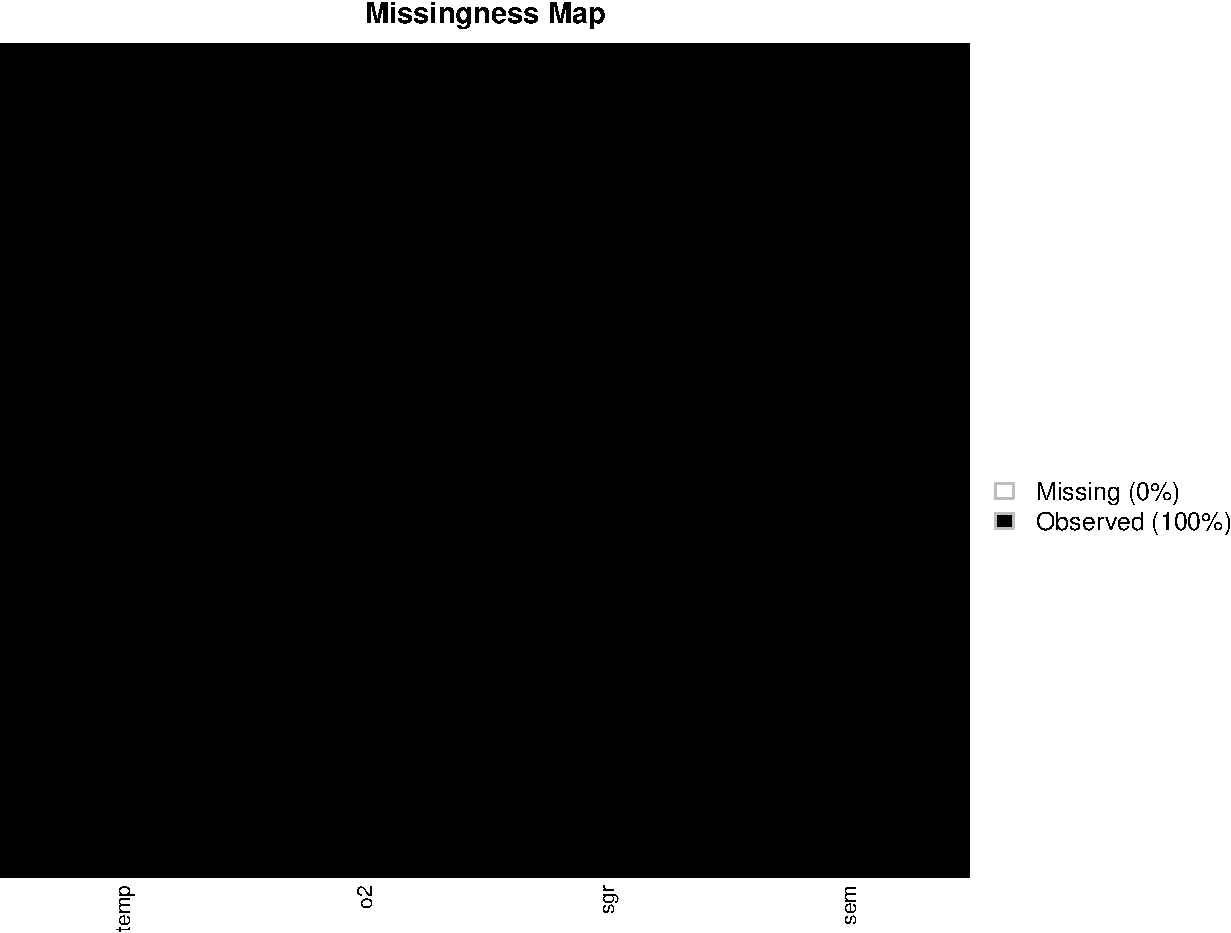
\includegraphics[width=0.7\linewidth]{Trabajo_final_Roberto-Teran_files/figure-latex/unnamed-chunk-3-1} \end{center}

se puede apreciar que no hay falta de datos

\hypertarget{graficas-incluidas}{%
\subsection{Graficas incluidas}\label{graficas-incluidas}}

Para data revisada se realiza y se busca la mejor correlacion entre las
variables

\begin{center}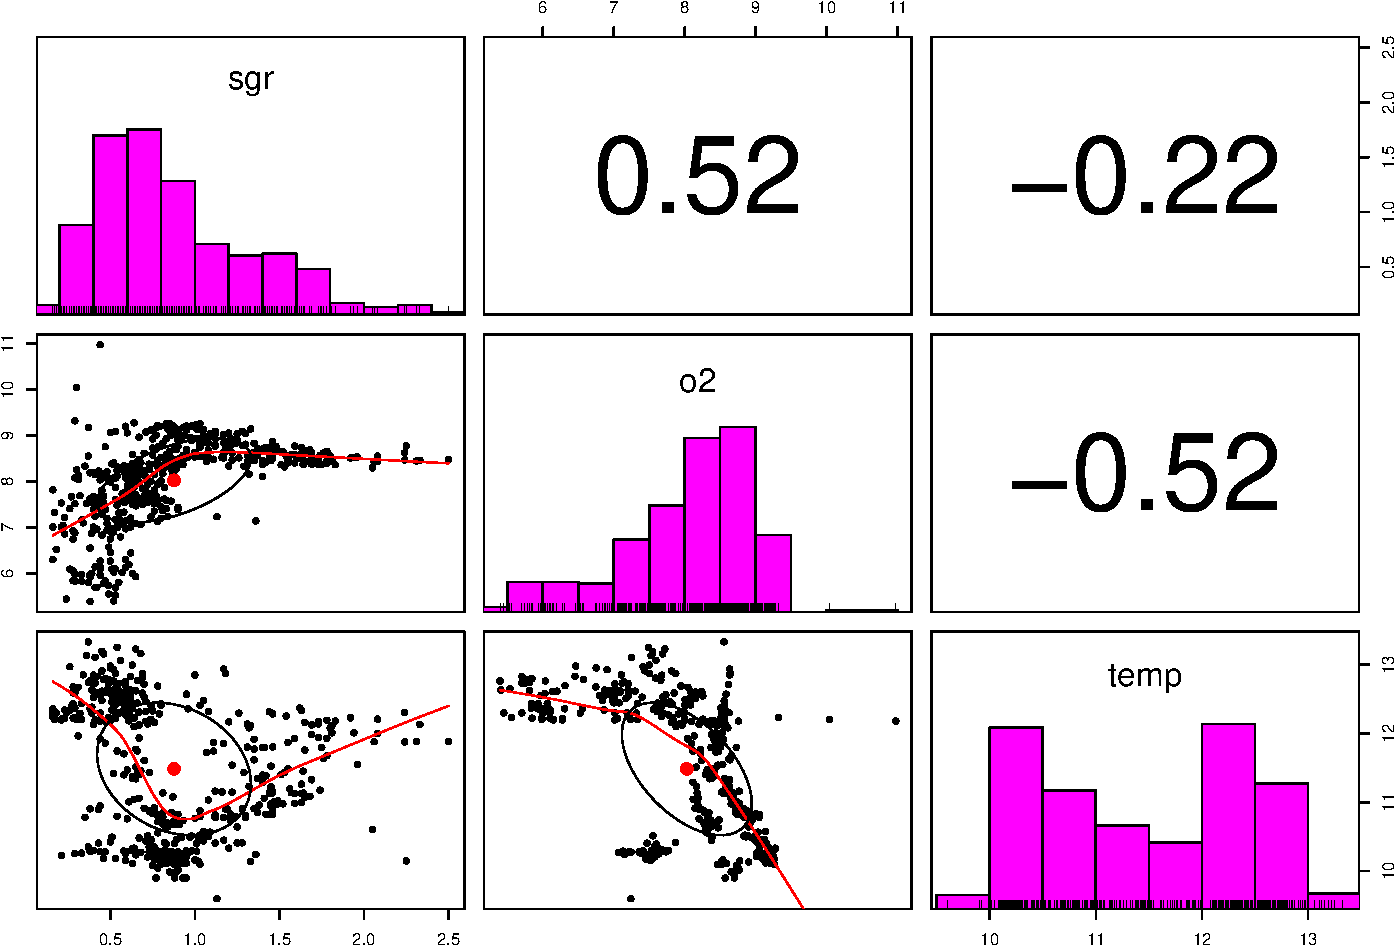
\includegraphics[width=0.6\linewidth]{Trabajo_final_Roberto-Teran_files/figure-latex/unnamed-chunk-4-1} \end{center}

al obtener una correlacion mas baja mediante Pearson intentaremos
mediante Spearman

\begin{Shaded}
\begin{Highlighting}[]
\NormalTok{P\_cor }\OtherTok{\textless{}{-}}\FunctionTok{cor.test}\NormalTok{(}\AttributeTok{x=}\NormalTok{rt}\SpecialCharTok{$}\NormalTok{sgr , }\AttributeTok{y=}\NormalTok{rt}\SpecialCharTok{$}\NormalTok{o2 , }\AttributeTok{method =} \StringTok{"pearson"}\NormalTok{, }\AttributeTok{conf.level =} \FloatTok{0.95}\NormalTok{)}
\NormalTok{pander}\SpecialCharTok{::}\FunctionTok{pander}\NormalTok{(P\_cor, }\AttributeTok{caption =} \StringTok{"Prueba de hipótesis para r entre Consumo bajo 20\% de centros con mayores consumos y FCRc."}\NormalTok{)}
\end{Highlighting}
\end{Shaded}

\begin{longtable}[]{@{}
  >{\centering\arraybackslash}p{(\columnwidth - 8\tabcolsep) * \real{0.2267}}
  >{\centering\arraybackslash}p{(\columnwidth - 8\tabcolsep) * \real{0.0800}}
  >{\centering\arraybackslash}p{(\columnwidth - 8\tabcolsep) * \real{0.2400}}
  >{\centering\arraybackslash}p{(\columnwidth - 8\tabcolsep) * \real{0.3333}}
  >{\centering\arraybackslash}p{(\columnwidth - 8\tabcolsep) * \real{0.1200}}@{}}
\caption{Prueba de hipótesis para r entre Consumo bajo 20\% de centros
con mayores consumos y FCRc.}\tabularnewline
\toprule
\begin{minipage}[b]{\linewidth}\centering
Test statistic
\end{minipage} & \begin{minipage}[b]{\linewidth}\centering
df
\end{minipage} & \begin{minipage}[b]{\linewidth}\centering
P value
\end{minipage} & \begin{minipage}[b]{\linewidth}\centering
Alternative hypothesis
\end{minipage} & \begin{minipage}[b]{\linewidth}\centering
cor
\end{minipage} \\
\midrule
\endfirsthead
\toprule
\begin{minipage}[b]{\linewidth}\centering
Test statistic
\end{minipage} & \begin{minipage}[b]{\linewidth}\centering
df
\end{minipage} & \begin{minipage}[b]{\linewidth}\centering
P value
\end{minipage} & \begin{minipage}[b]{\linewidth}\centering
Alternative hypothesis
\end{minipage} & \begin{minipage}[b]{\linewidth}\centering
cor
\end{minipage} \\
\midrule
\endhead
13.06 & 451 & 2.875e-33 * * * & two.sided & 0.5237 \\
\bottomrule
\end{longtable}

Buscamos relacion grafica

\begin{Shaded}
\begin{Highlighting}[]
\FunctionTok{ggplot}\NormalTok{(rt, }\FunctionTok{aes}\NormalTok{(}\AttributeTok{x=}\NormalTok{sgr, }\AttributeTok{y=}\NormalTok{o2)) }\SpecialCharTok{+} 
  \FunctionTok{geom\_point}\NormalTok{() }\SpecialCharTok{+} \FunctionTok{theme\_light}\NormalTok{()}
\end{Highlighting}
\end{Shaded}

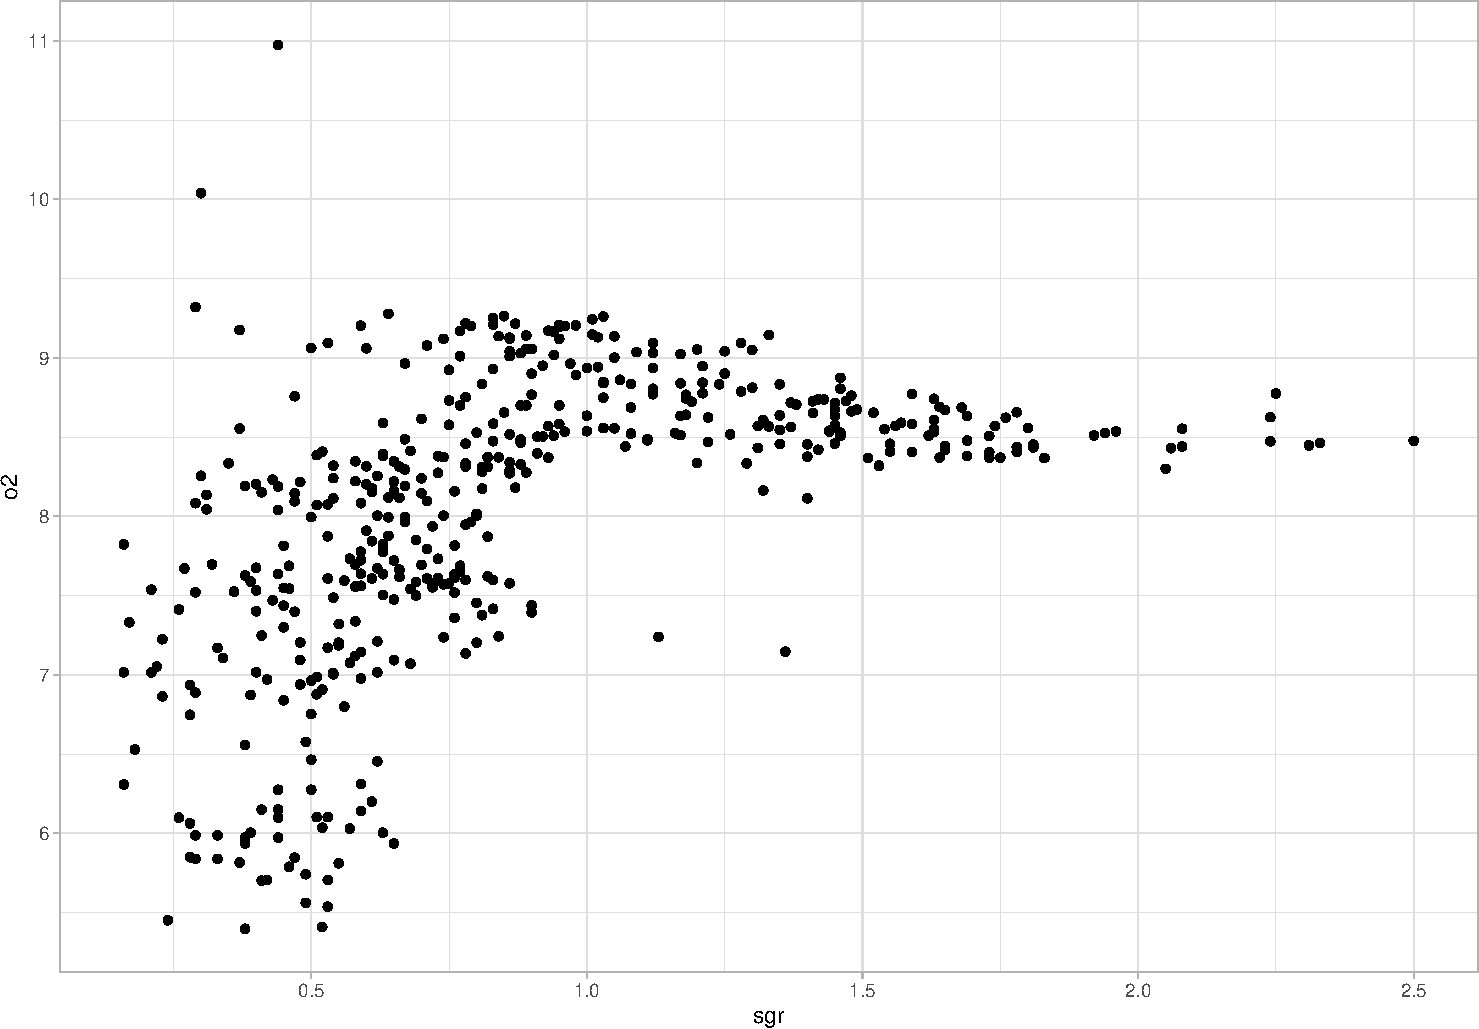
\includegraphics{Trabajo_final_Roberto-Teran_files/figure-latex/RT1-1.pdf}

\begin{Shaded}
\begin{Highlighting}[]
\FunctionTok{ggplot}\NormalTok{(rt, }\FunctionTok{aes}\NormalTok{(}\AttributeTok{x=}\NormalTok{sem, }\AttributeTok{y=}\NormalTok{o2)) }\SpecialCharTok{+} 
  \FunctionTok{geom\_point}\NormalTok{() }\SpecialCharTok{+} \FunctionTok{theme\_light}\NormalTok{()}
\end{Highlighting}
\end{Shaded}

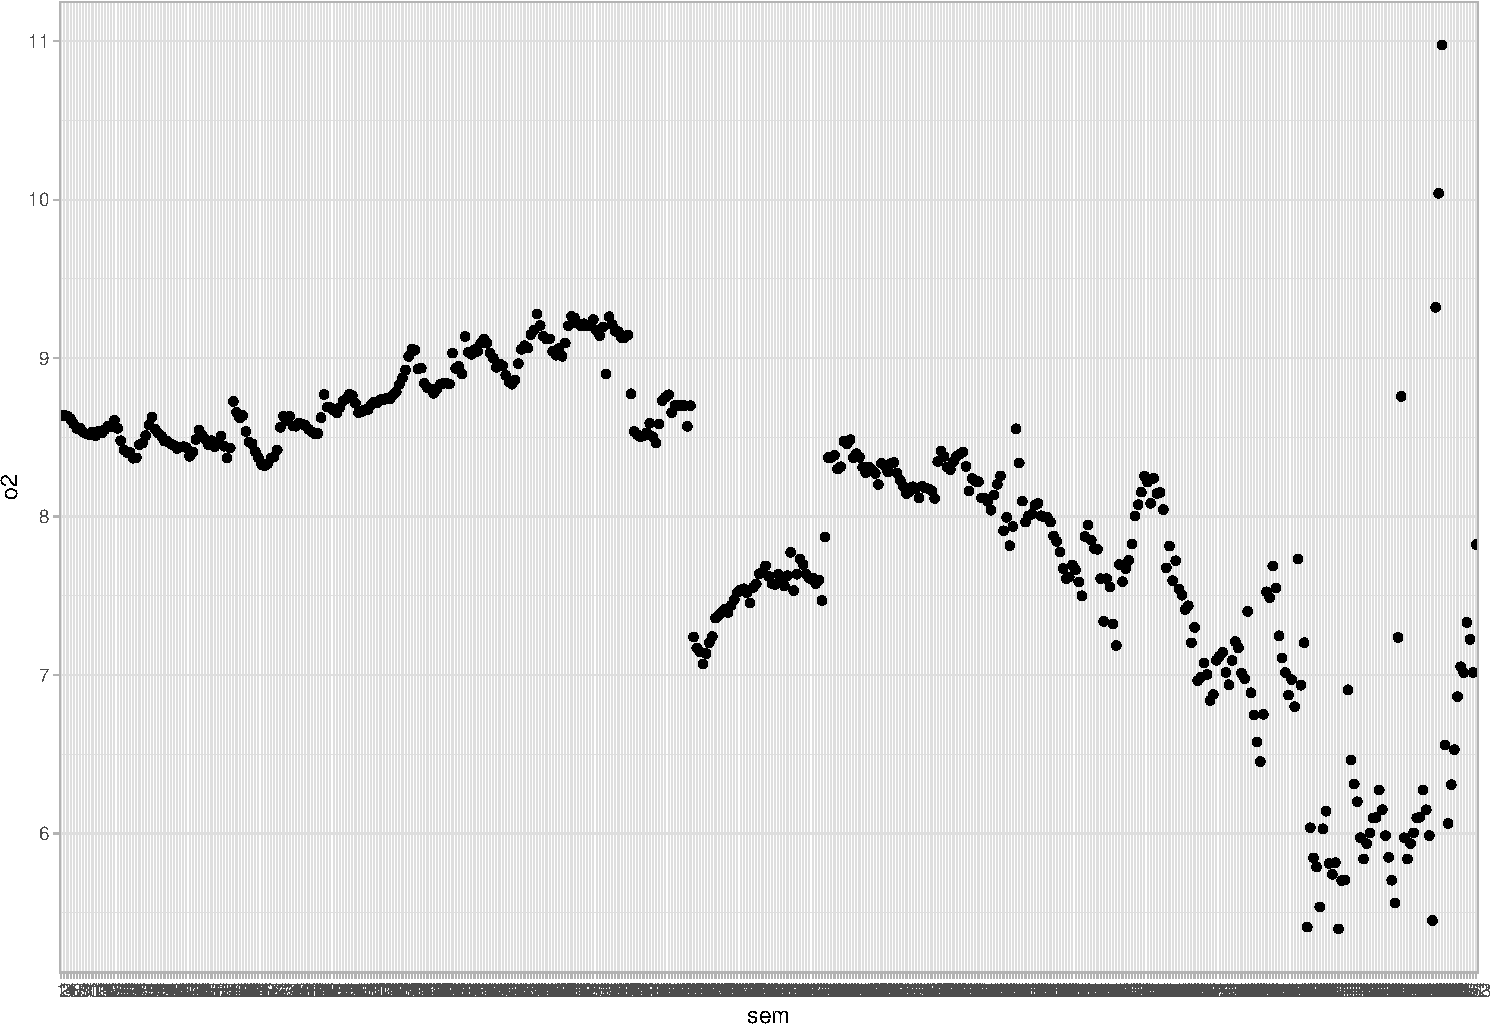
\includegraphics{Trabajo_final_Roberto-Teran_files/figure-latex/RT1-2.pdf}

\begin{Shaded}
\begin{Highlighting}[]
\FunctionTok{ggplot}\NormalTok{(rt, }\FunctionTok{aes}\NormalTok{(}\AttributeTok{x=}\NormalTok{sgr, }\AttributeTok{y=}\NormalTok{temp)) }\SpecialCharTok{+} 
  \FunctionTok{geom\_point}\NormalTok{() }\SpecialCharTok{+} \FunctionTok{theme\_light}\NormalTok{()}
\end{Highlighting}
\end{Shaded}

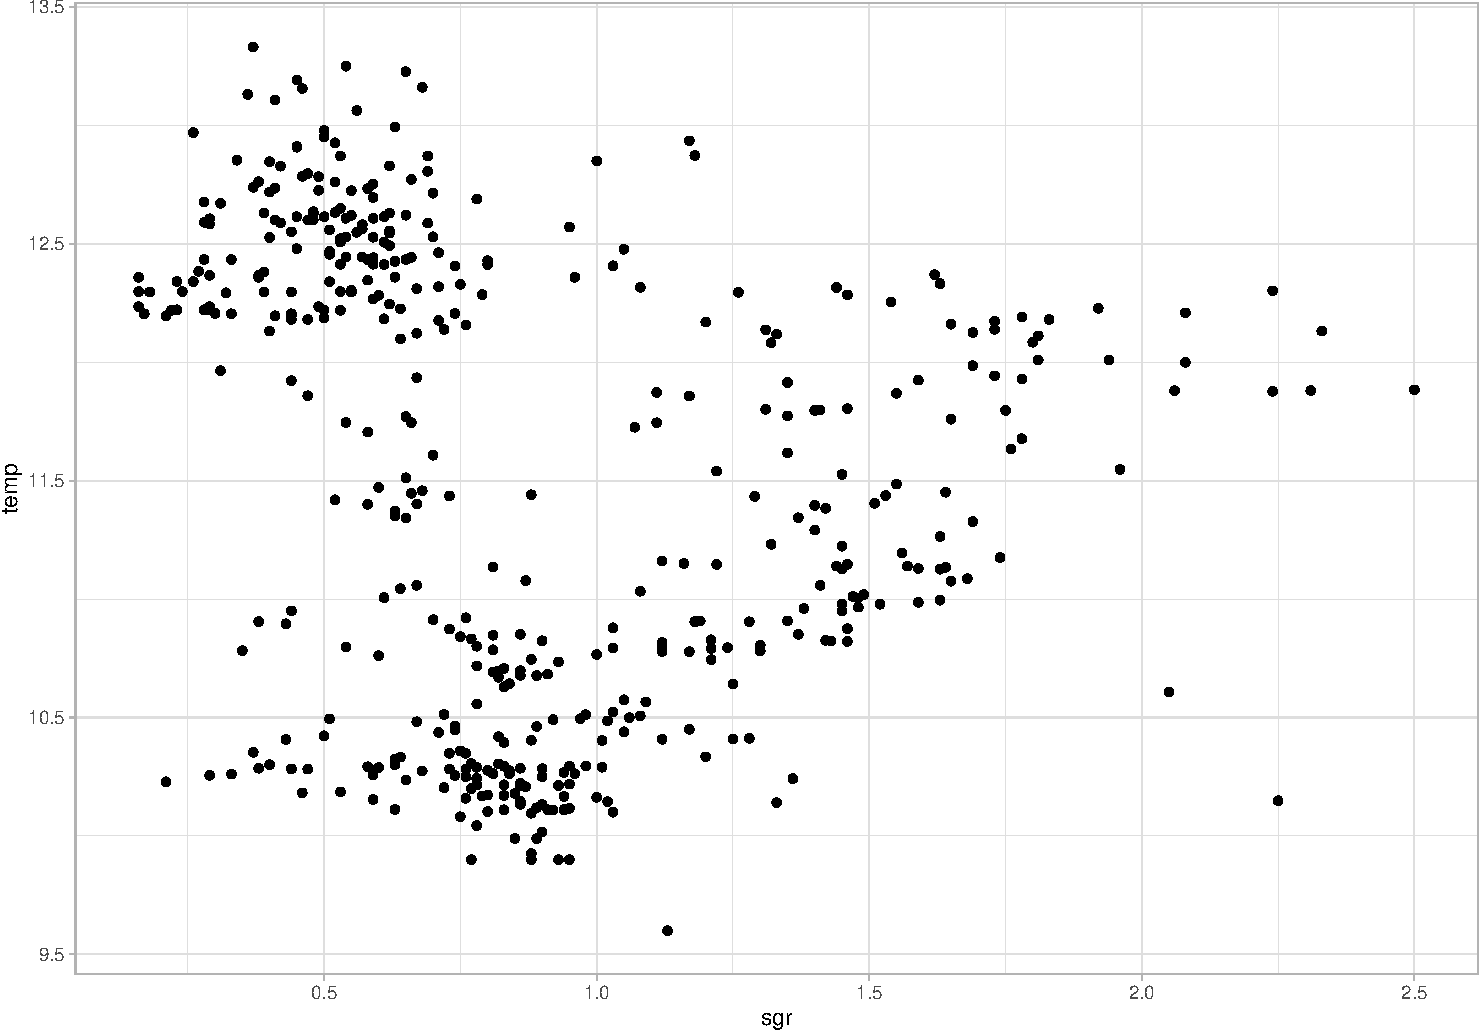
\includegraphics{Trabajo_final_Roberto-Teran_files/figure-latex/RT1-3.pdf}

Aun no puede darse una respuesta clara de cual podria ser la mejor
correlacion

\#\#Muestre el efecto de las variables independientes con respecto a la
variable dependiente.

\begin{verbatim}
## `geom_smooth()` using method = 'loess' and formula 'y ~ x'
\end{verbatim}

\begin{center}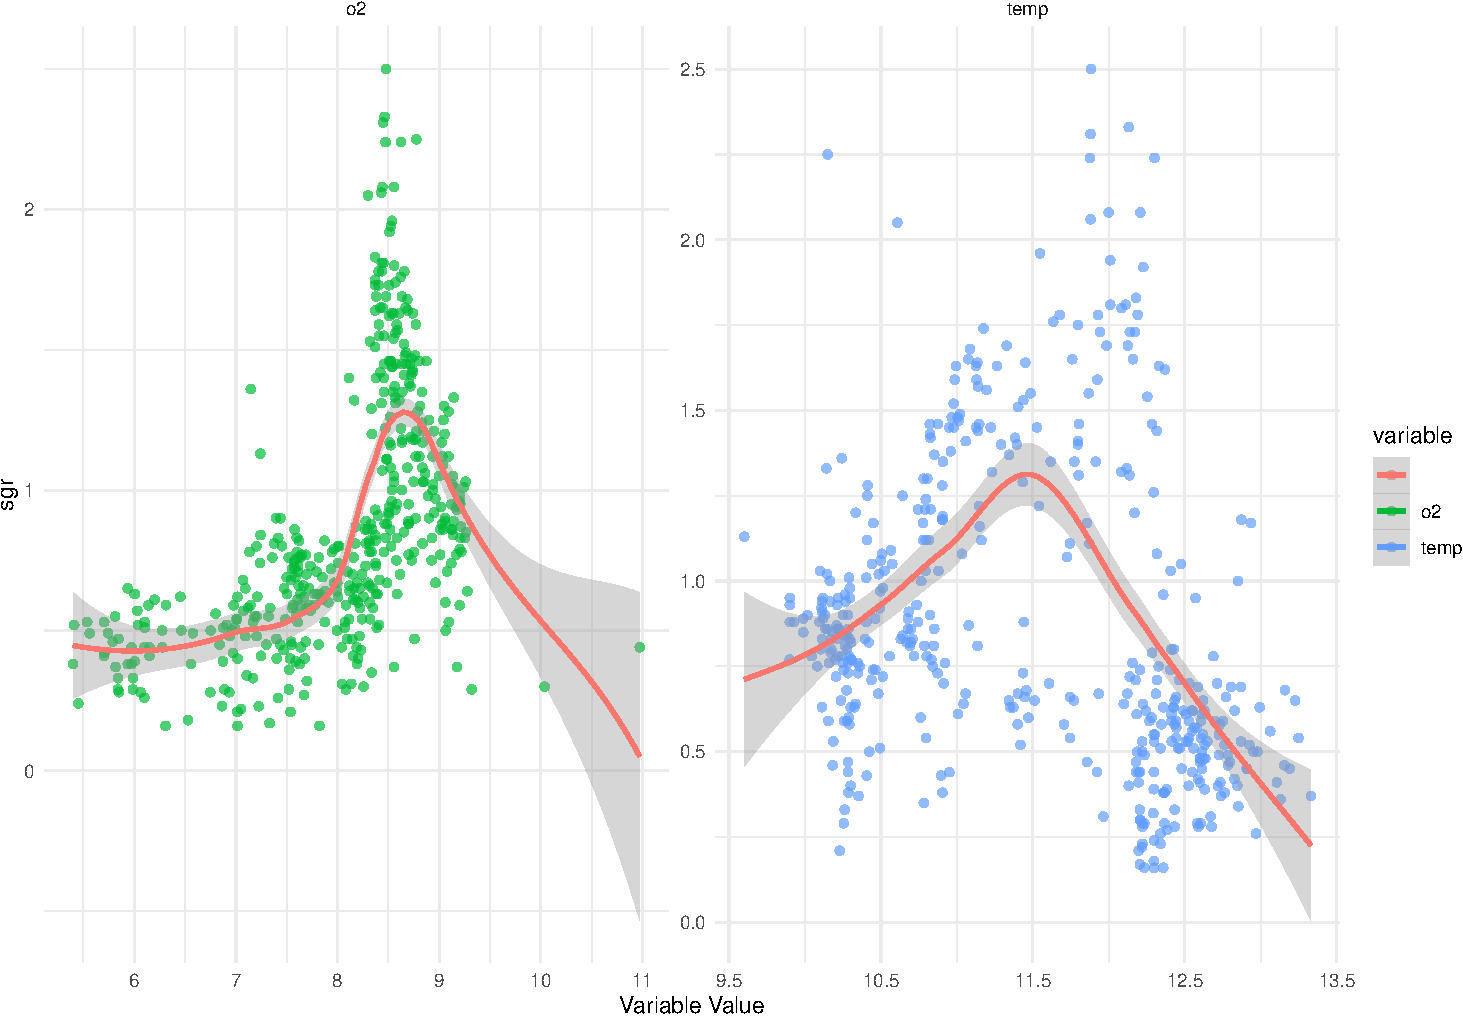
\includegraphics[width=0.7\linewidth]{Trabajo_final_Roberto-Teran_files/figure-latex/unnamed-chunk-7-1} \end{center}

La variable Sgr por lo que se puede ver es que depende claramente de O2
y temperatura .

\#\#obtendremos las estimaciones de los parametros estadisticos\#\#

\begin{verbatim}
## 
## Call:
## lm(formula = sgr ~ o2, data = rt)
## 
## Coefficients:
## (Intercept)           o2  
##     -1.2128       0.2602
\end{verbatim}

En la salida anterior se observan los valores estimados de ??0 y ??1
pero no aparece la estimacion de ?? Para obtener una tabla de resumen
con detalles del modelo ajustado, se usa la funcion generica summary

\begin{verbatim}
## 
## Call:
## lm(formula = sgr ~ o2, data = rt)
## 
## Residuals:
##      Min       1Q   Median       3Q      Max 
## -1.20260 -0.24981 -0.07131  0.16356  1.50738 
## 
## Coefficients:
##             Estimate Std. Error t value Pr(>|t|)    
## (Intercept) -1.21280    0.16107   -7.53  2.8e-13 ***
## o2           0.26020    0.01993   13.05  < 2e-16 ***
## ---
## Signif. codes:  0 '***' 0.001 '**' 0.01 '*' 0.05 '.' 0.1 ' ' 1
## 
## Residual standard error: 0.3881 on 451 degrees of freedom
## Multiple R-squared:  0.2743, Adjusted R-squared:  0.2727 
## F-statistic: 170.4 on 1 and 451 DF,  p-value: < 2.2e-16
\end{verbatim}

Para incluir la recta de regresion que representa el modelo ajustado
anterior\ldots{}

\begin{center}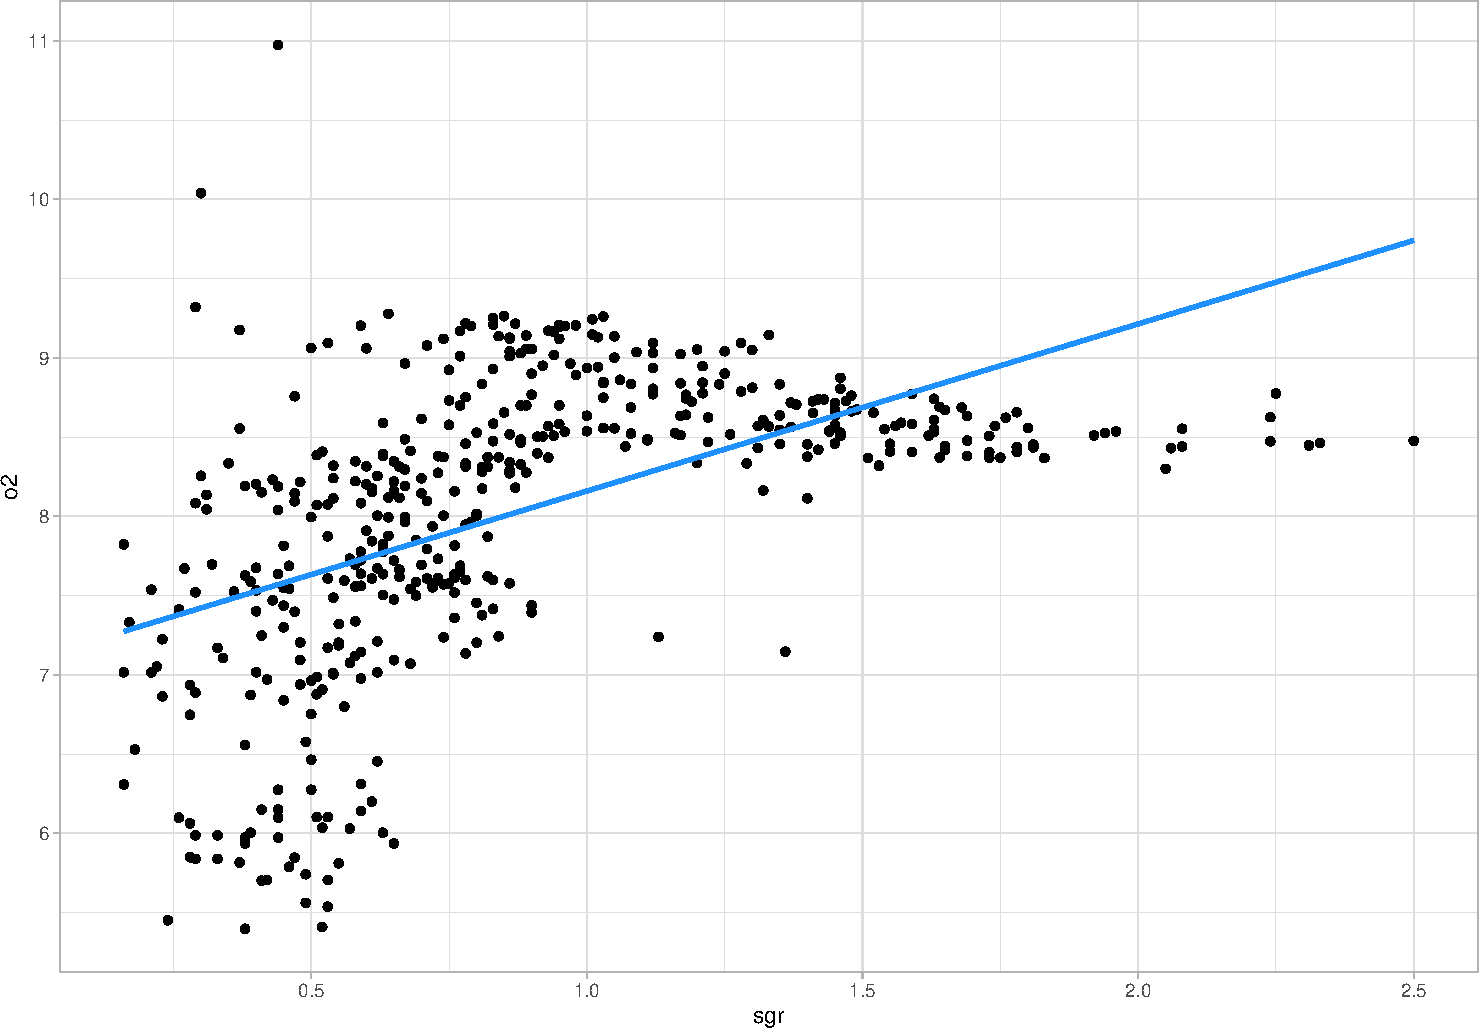
\includegraphics[width=0.7\linewidth]{Trabajo_final_Roberto-Teran_files/figure-latex/unnamed-chunk-10-1} \end{center}

\begin{center}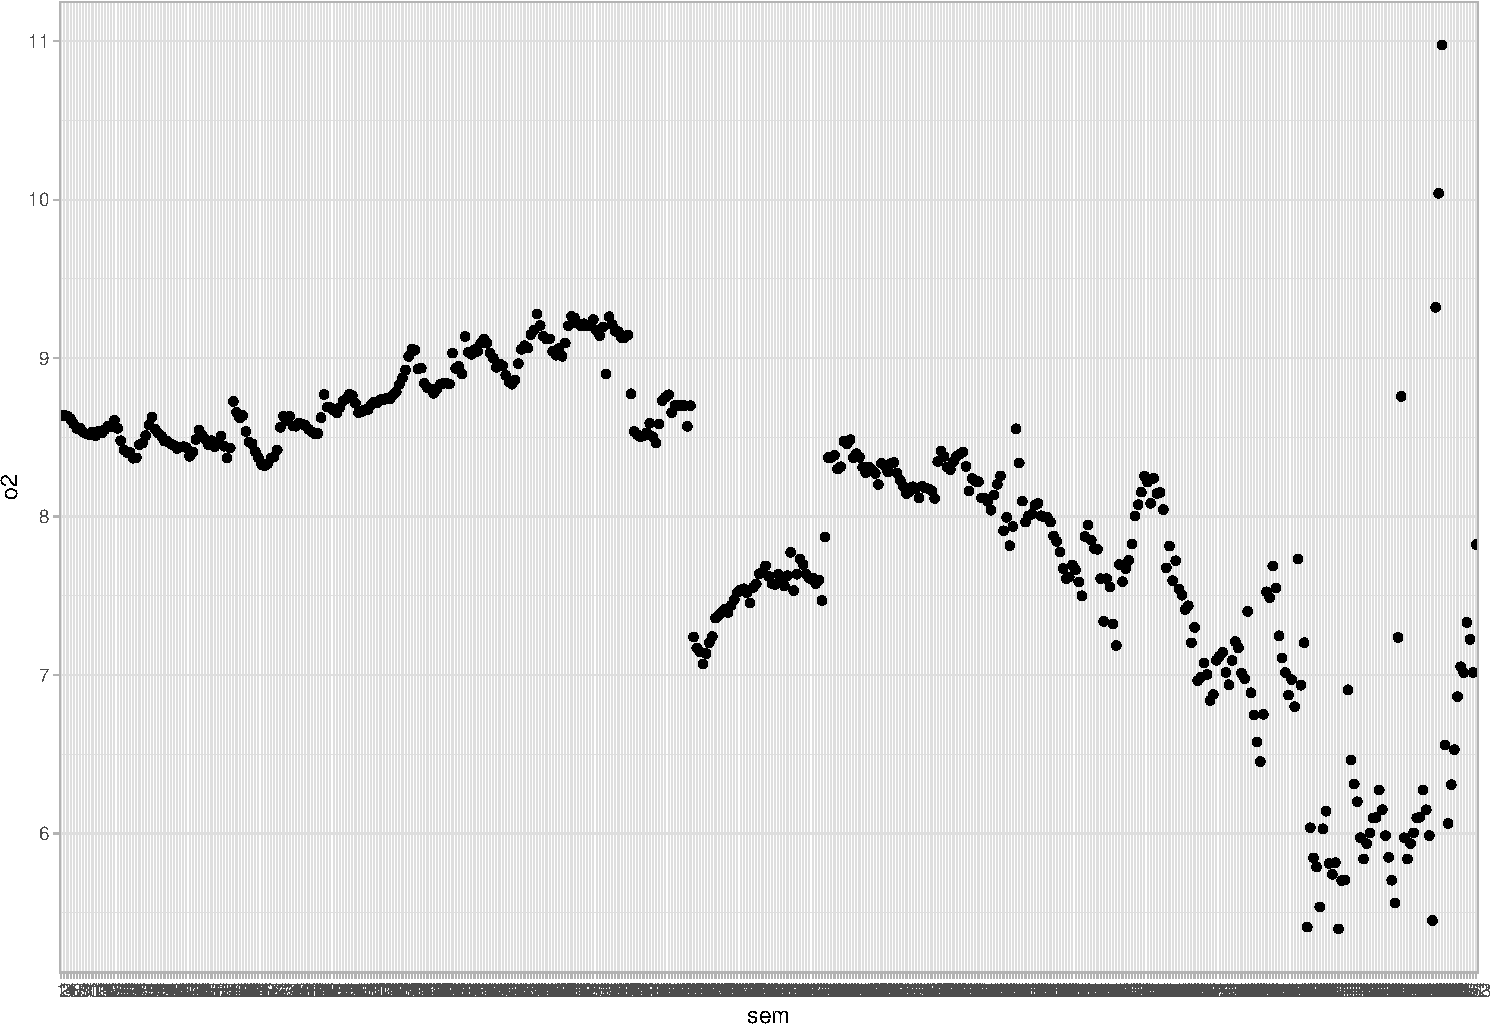
\includegraphics[width=0.7\linewidth]{Trabajo_final_Roberto-Teran_files/figure-latex/unnamed-chunk-10-2} \end{center}

\begin{center}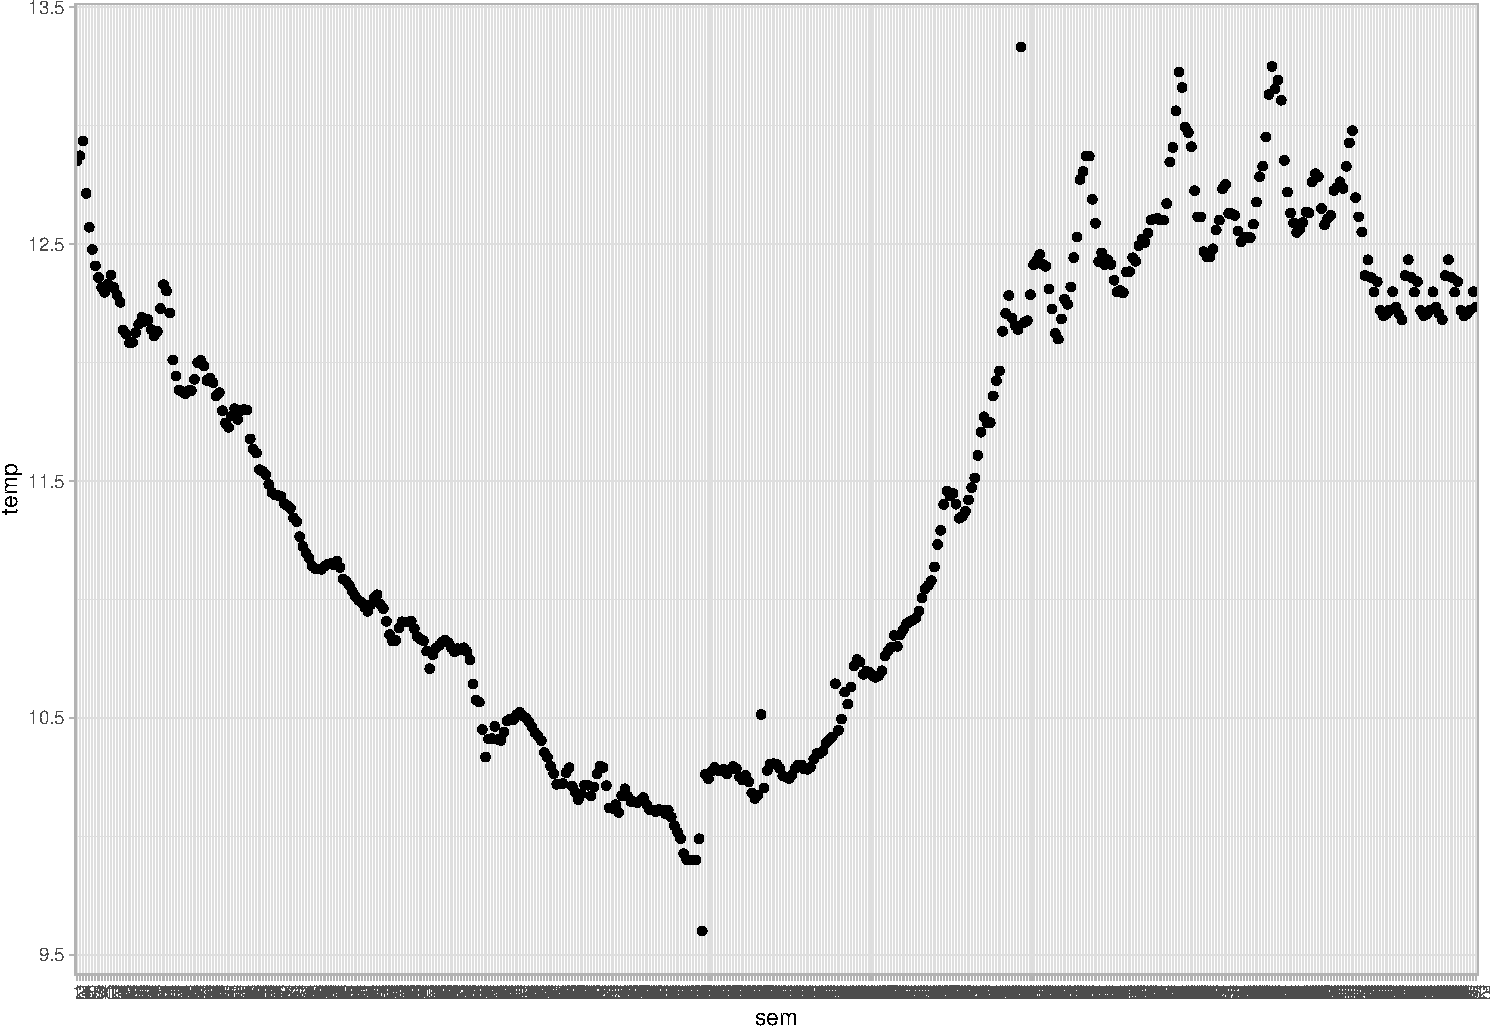
\includegraphics[width=0.7\linewidth]{Trabajo_final_Roberto-Teran_files/figure-latex/unnamed-chunk-10-3} \end{center}

la regresion lineal no se ajusta de buena manera a la nube de datos

utilizaremos regresion multiple

\begin{center}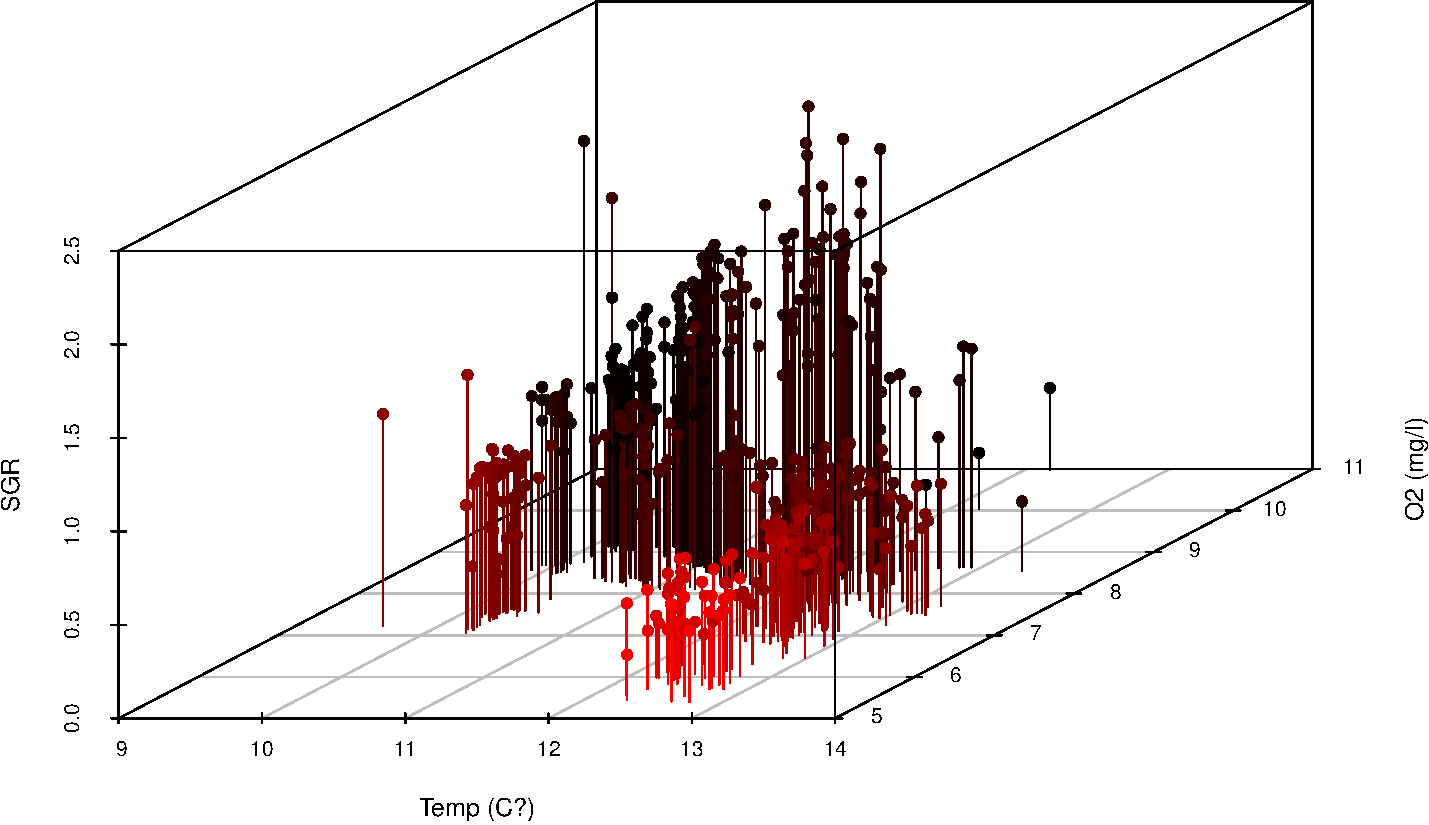
\includegraphics[width=0.7\linewidth]{Trabajo_final_Roberto-Teran_files/figure-latex/unnamed-chunk-11-1} \end{center}

a medida que aumenta la temperatura, aumenta el SGR y en condiciones de
mayor o2

\begin{verbatim}
## 
## Attaching package: 'plotly'
\end{verbatim}

\begin{verbatim}
## The following object is masked from 'package:MASS':
## 
##     select
\end{verbatim}

\begin{verbatim}
## The following object is masked from 'package:ggplot2':
## 
##     last_plot
\end{verbatim}

\begin{verbatim}
## The following object is masked from 'package:stats':
## 
##     filter
\end{verbatim}

\begin{verbatim}
## The following object is masked from 'package:graphics':
## 
##     layout
\end{verbatim}

\begin{verbatim}
## No scatter3d mode specifed:
##   Setting the mode to markers
##   Read more about this attribute -> https://plotly.com/r/reference/#scatter-mode
\end{verbatim}

\begin{verbatim}
## QStandardPaths: XDG_RUNTIME_DIR not set, defaulting to '/tmp/runtime-r1414764'
## TypeError: Attempting to change the setter of an unconfigurable property.
## TypeError: Attempting to change the setter of an unconfigurable property.
\end{verbatim}

\begin{center}
\includegraphics[width=0.7\linewidth]{Trabajo_final_Roberto-Teran_files/figure-latex/unnamed-chunk-12-1} \end{center}

la grafica anterior confirma los aprecia anteriormente, el color mas
claro muestra los puntos mas optimos.

\hypertarget{modelo-1}{%
\subsection{MOdelo 1}\label{modelo-1}}

\#basandonos en el modelo 3d, la expresion que se ajusta es:

\begin{center}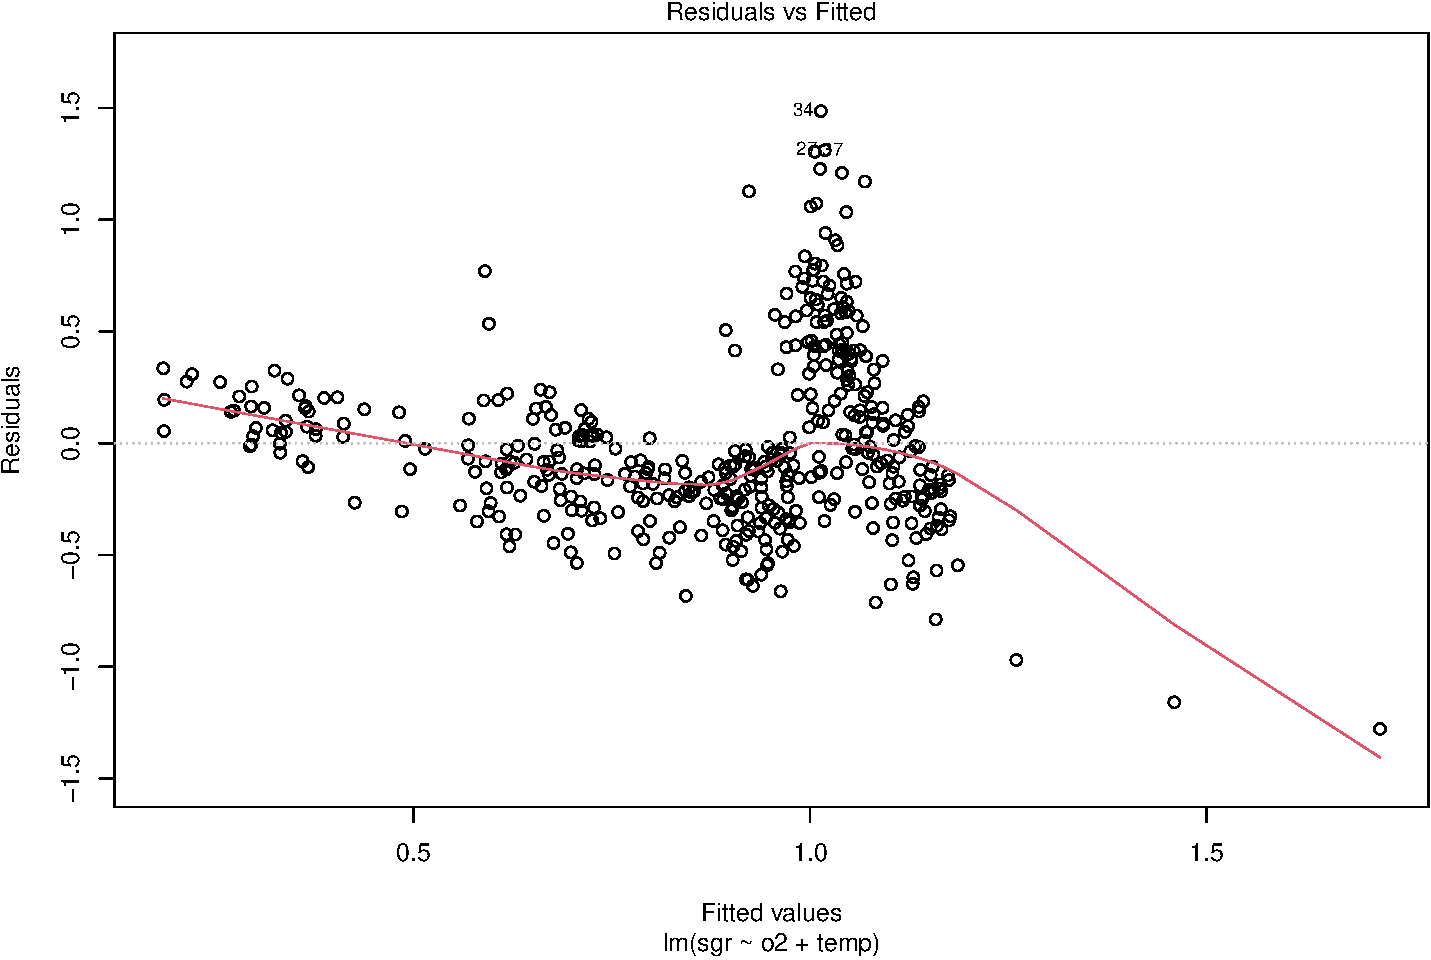
\includegraphics[width=0.7\linewidth]{Trabajo_final_Roberto-Teran_files/figure-latex/unnamed-chunk-13-1} \end{center}

\begin{center}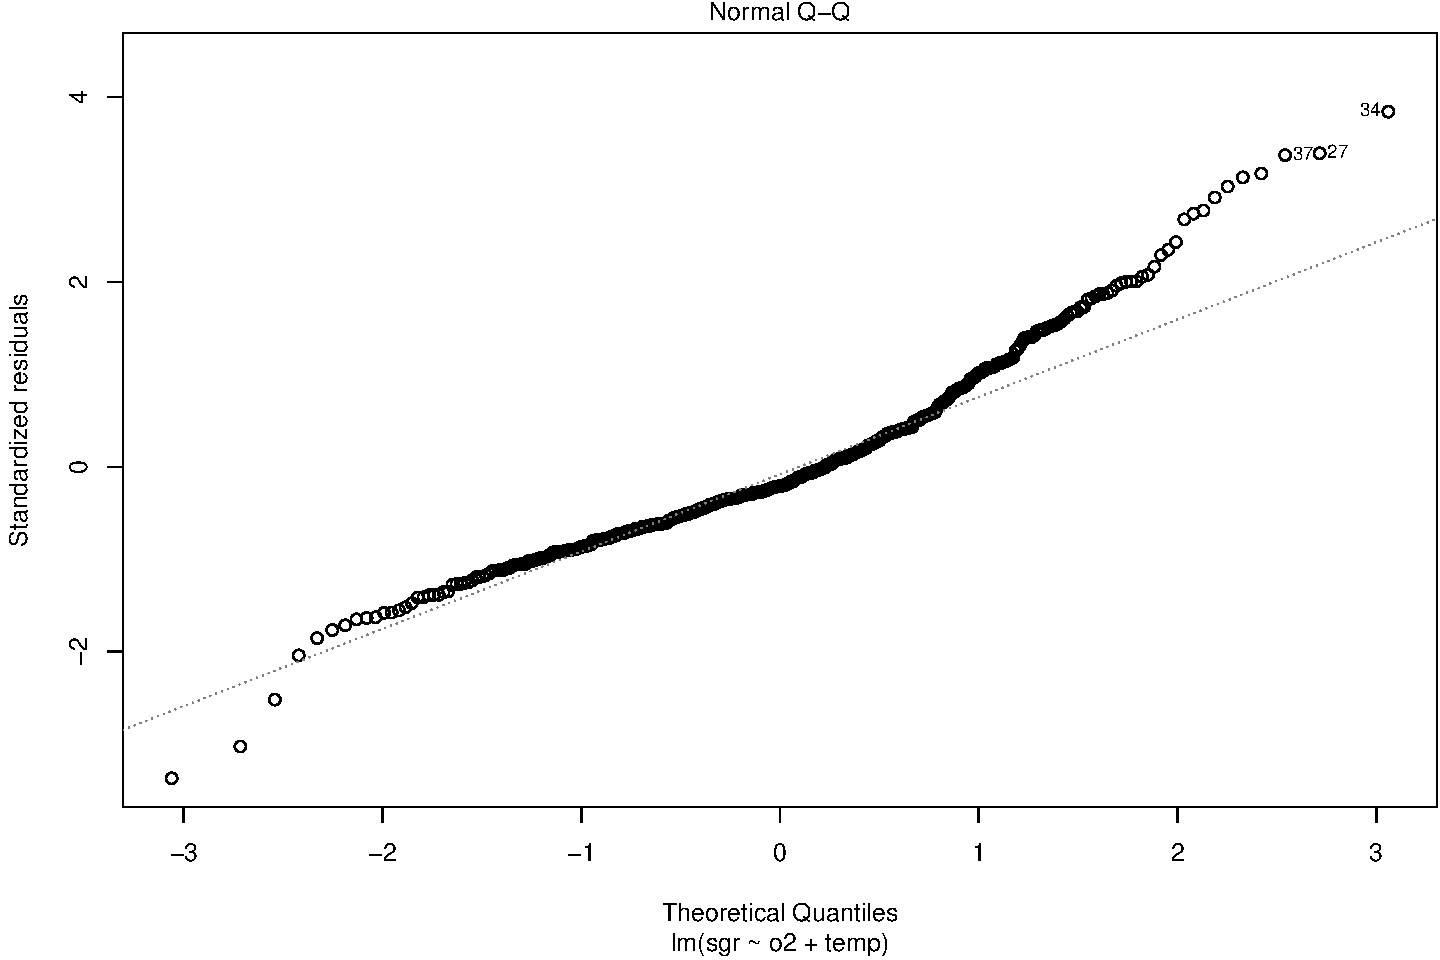
\includegraphics[width=0.7\linewidth]{Trabajo_final_Roberto-Teran_files/figure-latex/unnamed-chunk-13-2} \end{center}

\begin{center}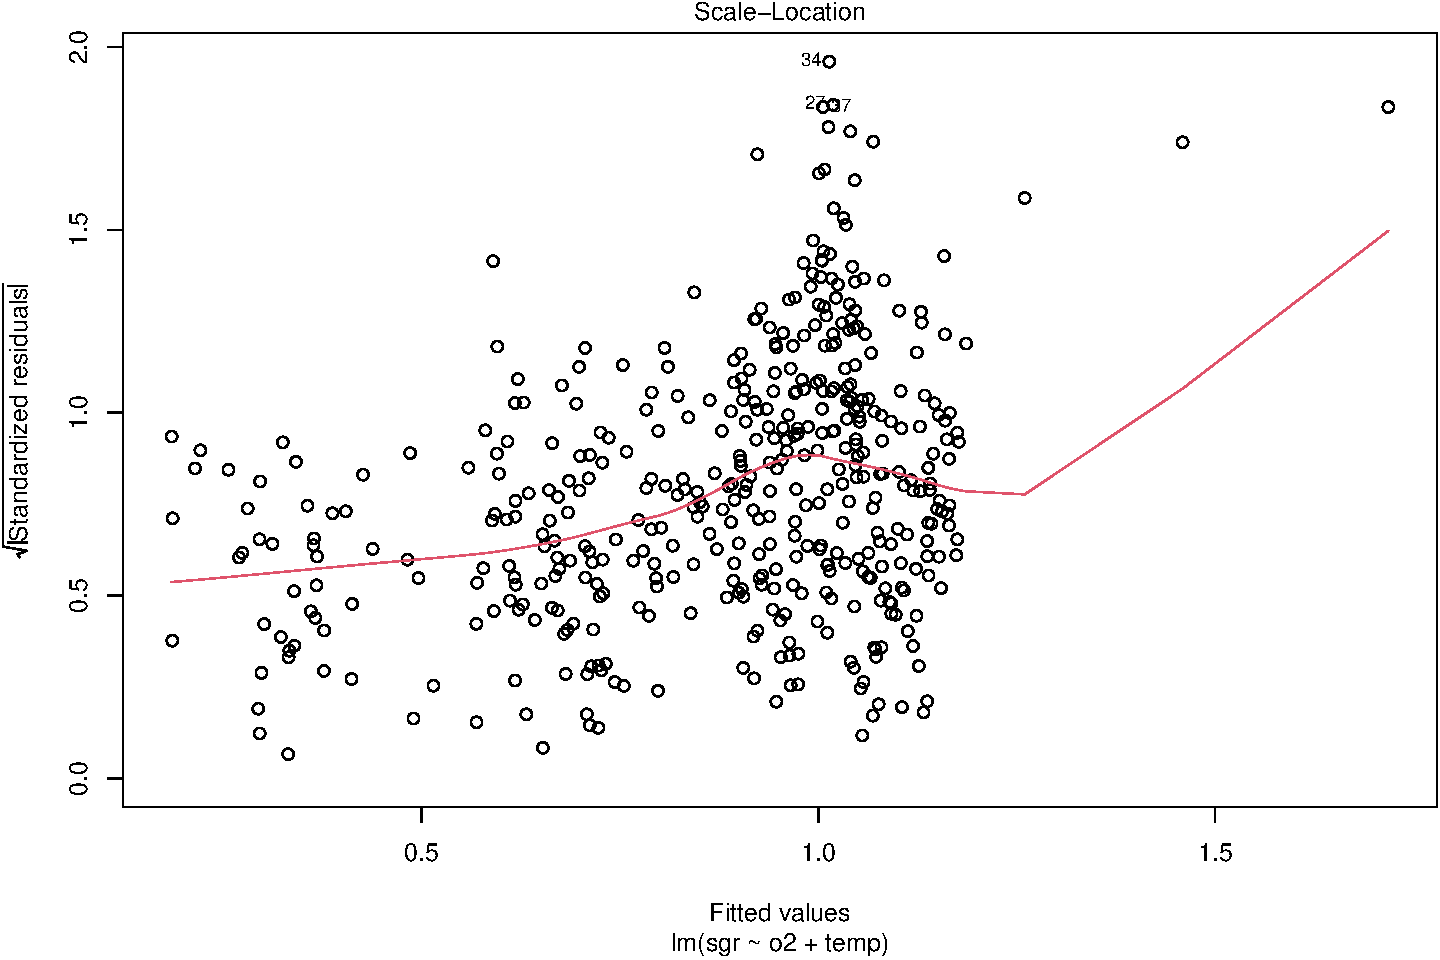
\includegraphics[width=0.7\linewidth]{Trabajo_final_Roberto-Teran_files/figure-latex/unnamed-chunk-13-3} \end{center}

\begin{center}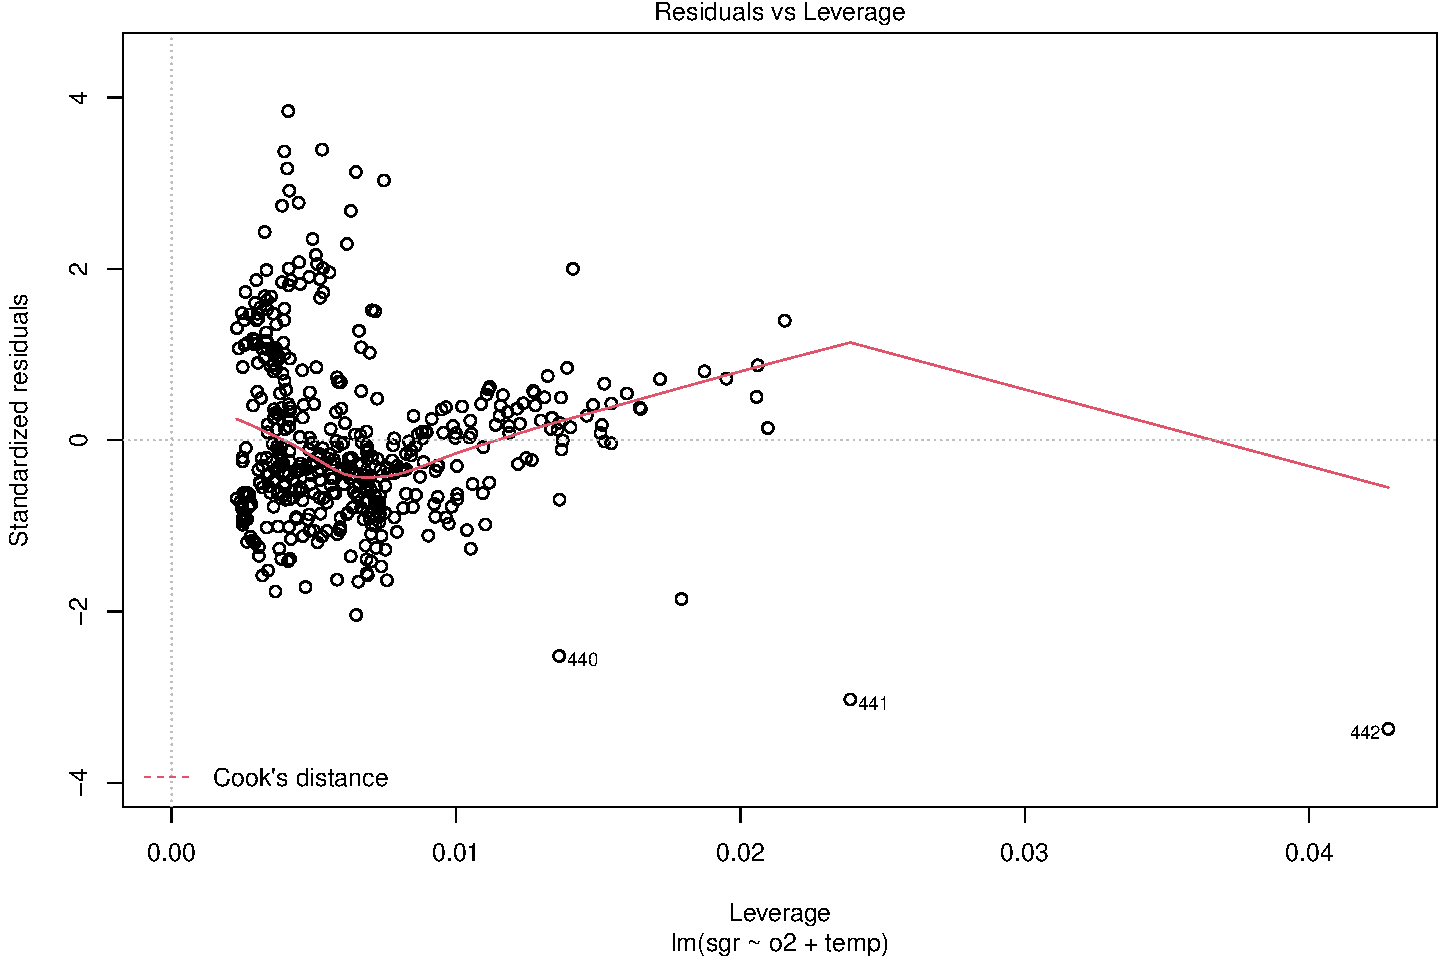
\includegraphics[width=0.7\linewidth]{Trabajo_final_Roberto-Teran_files/figure-latex/unnamed-chunk-13-4} \end{center}

\begin{verbatim}
## 
## Call:
## lm(formula = sgr ~ o2 + temp, data = rt)
## 
## Residuals:
##      Min       1Q   Median       3Q      Max 
## -1.27840 -0.24930 -0.08086  0.18735  1.48631 
## 
## Coefficients:
##             Estimate Std. Error t value Pr(>|t|)    
## (Intercept) -1.73268    0.38872  -4.457 1.05e-05 ***
## o2           0.27823    0.02338  11.898  < 2e-16 ***
## temp         0.03266    0.02223   1.469    0.143    
## ---
## Signif. codes:  0 '***' 0.001 '**' 0.01 '*' 0.05 '.' 0.1 ' ' 1
## 
## Residual standard error: 0.3876 on 450 degrees of freedom
## Multiple R-squared:  0.2777, Adjusted R-squared:  0.2745 
## F-statistic: 86.52 on 2 and 450 DF,  p-value: < 2.2e-16
\end{verbatim}

Para incluir el plano de regresion que representa el modelo ajustado
anterior

Se crea el grafico 3d y se guarda en un objeto, por ejemplo mi\_3d

\begin{center}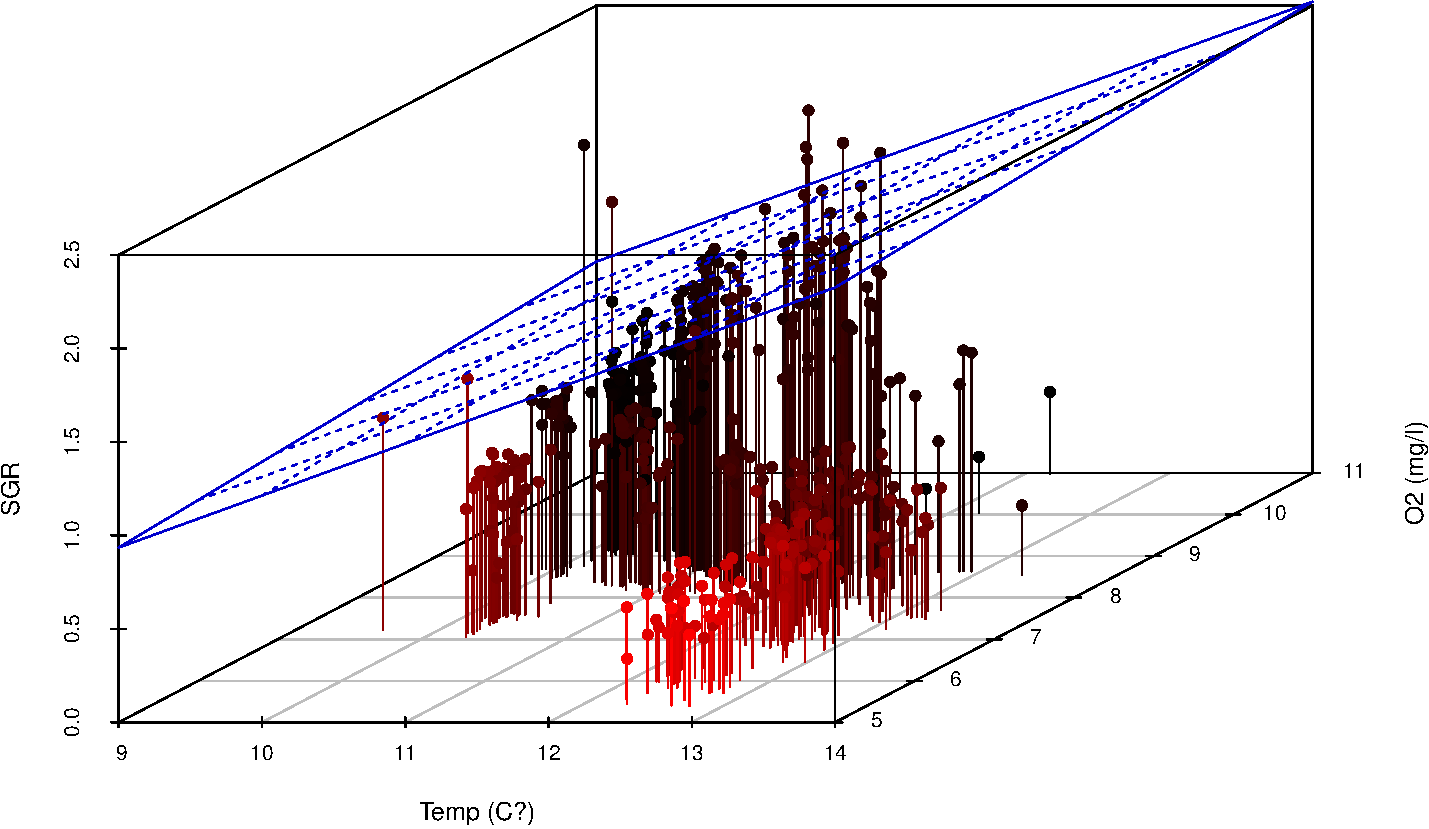
\includegraphics[width=0.7\linewidth]{Trabajo_final_Roberto-Teran_files/figure-latex/unnamed-chunk-14-1} \end{center}

podemos ver que en la grafica 3D la regresion se ajusta de mejor manera
los a ambas variables una dependeiente de la otra.

\begin{center}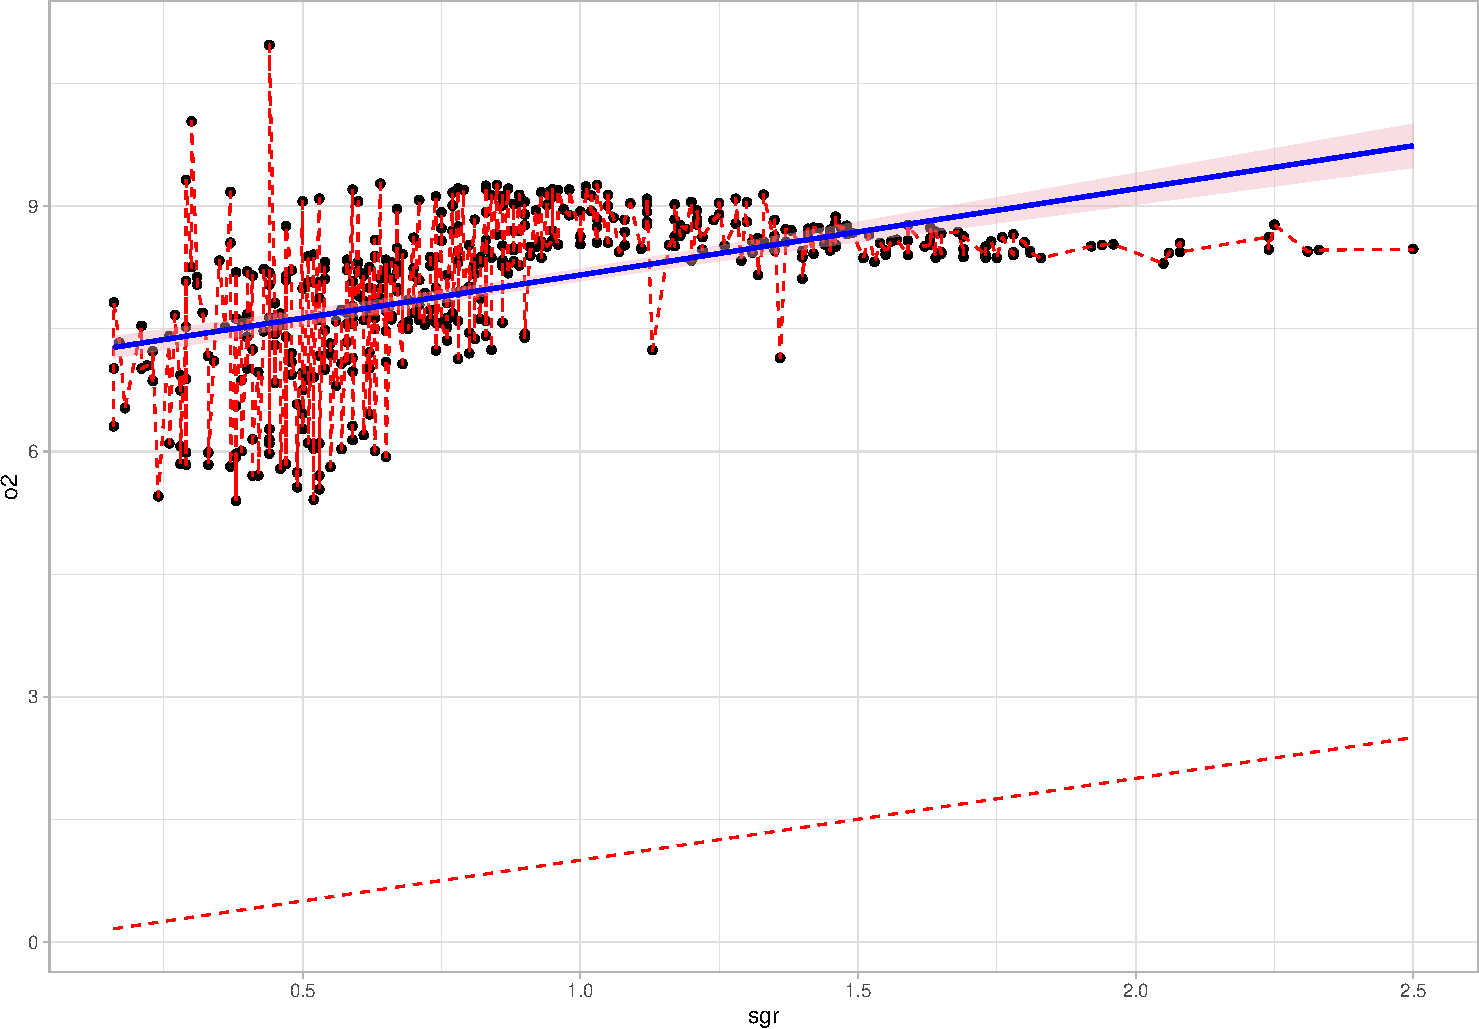
\includegraphics[width=0.7\linewidth]{Trabajo_final_Roberto-Teran_files/figure-latex/unnamed-chunk-15-1} \end{center}

haca ya llevamos a un plano la regresion mostrando la mejor concordancia
entre el O2 y el Sgr.

\#\#¿Que hipotesis contrasta la prueba de Kruskal-Wallis?

Ho: la variable respuesta es la misma en todas las variables valoradas

Ha: la variable respuesta es mayor en ciertos niveles.

\begin{Shaded}
\begin{Highlighting}[]
\FunctionTok{kruskal.test}\NormalTok{(rt}\SpecialCharTok{$}\NormalTok{sgr, rt}\SpecialCharTok{$}\NormalTok{temp)}
\end{Highlighting}
\end{Shaded}

\begin{verbatim}
## 
##  Kruskal-Wallis rank sum test
## 
## data:  rt$sgr and rt$temp
## Kruskal-Wallis chi-squared = 424.44, df = 384, p-value = 0.07565
\end{verbatim}

Indica cual es el estadistico de contraste, los grados de libertad, el
p-valor correspondiente y cual seria el valor critico que definiria las
regiones de aceptacion y rechazo con un nivel de significacion alfa =
0.1.

\begin{Shaded}
\begin{Highlighting}[]
\FunctionTok{qchisq}\NormalTok{(}\FloatTok{0.07}\NormalTok{, }\DecValTok{2{-}1}\NormalTok{, }\AttributeTok{lower.tail =}\NormalTok{ F)}\CommentTok{\#Valor teorico}
\end{Highlighting}
\end{Shaded}

\begin{verbatim}
## [1] 3.28302
\end{verbatim}

\#chi cuadrado es 436 \textgreater3.283 se acepta la Ho.

\begin{Shaded}
\begin{Highlighting}[]
\FunctionTok{kruskal.test}\NormalTok{(}\FunctionTok{log}\NormalTok{(rt}\SpecialCharTok{$}\NormalTok{sgr), rt}\SpecialCharTok{$}\NormalTok{temp) }\CommentTok{\#log para reducir escala de dispersión}
\end{Highlighting}
\end{Shaded}

\begin{verbatim}
## 
##  Kruskal-Wallis rank sum test
## 
## data:  log(rt$sgr) and rt$temp
## Kruskal-Wallis chi-squared = 424.44, df = 384, p-value = 0.07565
\end{verbatim}

Los resultados son exactamente los mismos. No se producen variaciones
porque el test de Kruskal-Wallis trabaja sobre rangos, es decir, sobre
ordenaciones de los valores de la variable en cada uno de los grupos.
Aunque realicemos una transformacion logaritmica, el orden entre los
valores de la variable se mantiene y por lo tanto la transformacion no
afecta a los resultados del test.

\hypertarget{nuevos-test}{%
\subsubsection{Nuevos test}\label{nuevos-test}}

se realizan nuevos test para analizar si poseemos una autocorrelacion en
los residuos de la regresion.

\begin{verbatim}
## 
##  Durbin-Watson test
## 
## data:  lm(sgr ~ o2 + temp, data = rt)
## DW = 0.54386, p-value < 2.2e-16
## alternative hypothesis: true autocorrelation is not 0
\end{verbatim}

\begin{verbatim}
## 
##  studentized Breusch-Pagan test
## 
## data:  lm(sgr ~ o2 + temp, data = rt)
## BP = 62.624, df = 2, p-value = 2.52e-14
\end{verbatim}

\begin{verbatim}
## 
##  Shapiro-Wilk normality test
## 
## data:  residuals(mod)
## W = 0.95352, p-value = 9.6e-11
\end{verbatim}

como vemos todos los P-value son bajos a 1 por lo cual se rechaza la
hipotesis de autocorrelacion del primer modelo por lo cual generaremos
nuevas iteraciones. por ende se concluye que lo anterior no se
distribuye de manera normal. a lo anterior recurrieremos a modelos
multivariables

\hypertarget{modelo-2}{%
\subsection{Modelo 2}\label{modelo-2}}

Provaremos una nueva variente del modelo (mod)

SGR = o2 \textasciitilde{} temp + (1\textbar{} semana)

\begin{Shaded}
\begin{Highlighting}[]
\NormalTok{mod2}\OtherTok{\textless{}{-}} \FunctionTok{lmer}\NormalTok{(sgr }\SpecialCharTok{\textasciitilde{}}\NormalTok{ o2 }\SpecialCharTok{+}\NormalTok{ (}\DecValTok{1} \SpecialCharTok{|}\NormalTok{ temp), }\AttributeTok{data =}\NormalTok{ rt)}
\FunctionTok{summary}\NormalTok{(mod2)}
\end{Highlighting}
\end{Shaded}

\begin{verbatim}
## Linear mixed model fit by REML ['lmerMod']
## Formula: sgr ~ o2 + (1 | temp)
##    Data: rt
## 
## REML criterion at convergence: 436
## 
## Scaled residuals: 
##     Min      1Q  Median      3Q     Max 
## -3.0078 -0.6109 -0.1711  0.4108  3.4975 
## 
## Random effects:
##  Groups   Name        Variance Std.Dev.
##  temp     (Intercept) 0.02829  0.1682  
##  Residual             0.12267  0.3502  
## Number of obs: 453, groups:  temp, 385
## 
## Fixed effects:
##             Estimate Std. Error t value
## (Intercept) -1.12598    0.16784  -6.709
## o2           0.24994    0.02068  12.086
## 
## Correlation of Fixed Effects:
##    (Intr)
## o2 -0.994
\end{verbatim}

\begin{Shaded}
\begin{Highlighting}[]
\FunctionTok{tab\_model}\NormalTok{(mod2, }\AttributeTok{show.se =} \ConstantTok{TRUE}\NormalTok{, }\AttributeTok{show.aic=}\ConstantTok{TRUE}\NormalTok{)}
\end{Highlighting}
\end{Shaded}

~

sgr

Predictors

Estimates

std. Error

CI

p

(Intercept)

-1.13

0.17

-1.46~--~-0.80

\textless0.001

o2

0.25

0.02

0.21~--~0.29

\textless0.001

Random Effects

σ2

0.12

τ00 temp

0.03

ICC

0.19

N temp

385

Observations

453

Marginal R2 / Conditional R2

0.258 / 0.397

AIC

443.966

\hypertarget{conclusiones}{%
\subsubsection{Conclusiones}\label{conclusiones}}

Se aprecia que hay una realcion estrecha ademas de la temperatura en el
crecimiento de los peces gatillado por las fluctuaciones del O2

\hypertarget{variable-no-se-distibuye-normal}{%
\subsection{variable no se distibuye
normal}\label{variable-no-se-distibuye-normal}}

MLM

\hypertarget{otro}{%
\subsection{otro}\label{otro}}

\begin{Shaded}
\begin{Highlighting}[]
\NormalTok{mod3}\OtherTok{\textless{}{-}} \FunctionTok{lmer}\NormalTok{(sgr }\SpecialCharTok{\textasciitilde{}}\NormalTok{ temp }\SpecialCharTok{+}\NormalTok{ (}\DecValTok{1} \SpecialCharTok{|}\NormalTok{ o2), }\AttributeTok{data =}\NormalTok{ rt)}
\FunctionTok{summary}\NormalTok{(mod3)}
\end{Highlighting}
\end{Shaded}

\begin{verbatim}
## Linear mixed model fit by REML ['lmerMod']
## Formula: sgr ~ temp + (1 | o2)
##    Data: rt
## 
## REML criterion at convergence: 547
## 
## Scaled residuals: 
##     Min      1Q  Median      3Q     Max 
## -1.6572 -0.4607 -0.2456  0.3722  3.2844 
## 
## Random effects:
##  Groups   Name        Variance Std.Dev.
##  o2       (Intercept) 0.08685  0.2947  
##  Residual             0.10998  0.3316  
## Number of obs: 453, groups:  o2, 401
## 
## Fixed effects:
##             Estimate Std. Error t value
## (Intercept)  1.94026    0.25220   7.693
## temp        -0.09279    0.02187  -4.242
## 
## Correlation of Fixed Effects:
##      (Intr)
## temp -0.996
\end{verbatim}

\begin{Shaded}
\begin{Highlighting}[]
\FunctionTok{tab\_model}\NormalTok{(mod3, }\AttributeTok{show.se =} \ConstantTok{TRUE}\NormalTok{, }\AttributeTok{show.aic=}\ConstantTok{TRUE}\NormalTok{)}
\end{Highlighting}
\end{Shaded}

~

sgr

Predictors

Estimates

std. Error

CI

p

(Intercept)

1.94

0.25

1.44~--~2.44

\textless0.001

temp

-0.09

0.02

-0.14~--~-0.05

\textless0.001

Random Effects

σ2

0.11

τ00 o2

0.09

ICC

0.44

N o2

401

Observations

453

Marginal R2 / Conditional R2

0.039 / 0.463

AIC

554.996

\end{document}
